\documentclass[11pt]{article}
\usepackage[italian]{babel}
\usepackage[dvipsnames,table]{xcolor}
\usepackage{graphicx}
\usepackage{tabularx}
\usepackage{svg}
\usepackage{tikz}
\usepackage{amsmath}
\usepackage{blindtext}
\usepackage{booktabs}
\usepackage[a4paper,top=2cm,bottom=2cm,left=2cm,right=2cm,marginparwidth=1.75cm]{geometry}
\usepackage[colorlinks=true, allcolors=blue]{hyperref}
\usepackage{longtable}
\usepackage{makecell}
\usepackage{lscape}
\usepackage[final]{pdfpages}
\usetikzlibrary{arrows,shapes,positioning,shadows,trees}

\tikzset{
every node/.style={draw,text width=2.5cm,drop shadow},
style1/.style= {rectangle, rounded corners=2pt, thin,align=center,fill=Secondary},
style2/.style= {rectangle, rounded corners=6pt, thin,align=center,fill=Secondary!80},
style3/.style= {rectangle,thin,align=left,fill=Secondary!30},
node distance = 1.5cm
}

\renewcommand{\arraystretch}{1.5}

\definecolor{Primary}{HTML}{DC2626}
\definecolor{Secondary}{HTML}{FFFFFF}

\author{
Giorgio Matacera\\
\texttt{mataceragiorgio@gmail.com}
}
\title{\huge DressCode}
\date{\vspace{-5ex}}

\begin{document}
\maketitle
\begin{center}
    
\includegraphics[width=\linewidth]{logo.jpg}
\end{center}
\clearpage
{ \hypersetup{hidelinks} \tableofcontents }
\clearpage

\section{\huge Introduzione}
\subsection{Scopo del Documento}
Con questo documento si formalizza la fase di definizione e pianificazione progettuale per l'applicativo web \textbf{DressCode}. L'obiettivo principale è fornire una visione chiara e strutturata del progetto\\ \textbf{DressCode}, definendo le caratteristiche, le tempistiche e le strategie operative necessarie per lo sviluppo di un form builder innovativo e user-friendly.

\subsection{L'Idea e gli Obiettivi}
L'idea di \textbf{DressCode} è permettere agli utenti di costruire moduli personalizzati (form) integrabili in siti web o applicazioni esterne, senza richiedere competenze tecniche avanzate. Il progetto si basa su un'interfaccia intuitiva con un tema ispirato all'abbigliamento, che rende l'esperienza creativa e coinvolgente. Gli obiettivi principali sono:
\begin{itemize}
    \item[] \textbf{Semplificare la creazione di form:} Offrire uno strumento accessibile per progettare moduli complessi.
    \item[] \textbf{Promuovere la personalizzazione:} Fornire opzioni per adattare i form alle esigenze specifiche degli utenti.
    \item[] \textbf{Integrazione facile:} Consentire l'inserimento dei form in piattaforme esterne con semplicità.
\end{itemize}

\subsection{Il Team}
\ttfamily\large\begin{tabularx}{\linewidth}{lXr}
    Giorgio Matacera & & Designer UX, Sviluppatore full stack e Project Manager\\
\end{tabularx}
\rmfamily
% Aggiungi altri membri del team se necessario

\subsection{Analisi Tecnica}
Il progetto è tecnicamente fattibile, utilizzando tecnologie comuni e accessibili. Il tema dell'abbigliamento influenza solo l'interfaccia e la terminologia, senza complicare lo sviluppo.

\subsubsection{Tecnologie Necessarie}
\subsubsection*{Linguaggi di Programmazione e Markup}
\begin{itemize}
    \item HTML, CSS, JavaScript/TypeScript per il front-end;
    \item Typescript per il back-end;
    \item PostgreSQL per la base dati.
\end{itemize}

\subsubsection*{Software di Progettazione e Design}
\begin{itemize}
    \item Figma per wireframe, mockup e prototipazione;
\end{itemize}

\subsubsection*{Software per lo Sviluppo}
\begin{itemize}
    \item Neovim, WebStorm per la scrittura del codice.
\end{itemize}

\subsubsection*{Frameworks}
\begin{itemize}
    \item Angular full stack con render ibrido;
\end{itemize}

\subsubsection{Infrastruttura}
Il progetto richiederà un servizio di hosting per l'applicativo e il database, con scalabilità per gestire un numero crescente di utenti. Sarà necessario un dominio (es. DressCode.com) e un certificato SSL per la sicurezza.

\subsubsection{Sicurezza \& Privacy}
\textbf{DressCode} rispetterà il GDPR per la gestione dei dati degli utenti. Saranno inclusi termini e condizioni, una politica sulla privacy e misure di sicurezza (es. crittografia) per proteggere i dati raccolti dai form.

\subsection{Fattibilità Temporale}
La fattibilità temporale dipende dalle scadenze del corso. Con una metodologia agile e una pianificazione attenta, il progetto può essere completato entro il termine, anche se potrebbero esserci rischi di ritardi.

\subsection{Deliverable}
\begin{itemize}
  \item Prototipo interattivo di DressCode (realizzato in Angular).
  \item Documentazione completa (questo documento).
  \item Wireframe e mockup (in Figma).
\end{itemize}

\section{\huge Pianificazione Preliminare}
\subsection{Work Breakdown Structure (WBS)}
\begin{tikzpicture}[
remember picture,
level 1/.style={sibling distance=40mm},
edge from parent/.style={->,draw},
>=latex]
\node[style1] {DressCode}
child {node[style2] (c1) {Analisi}}
child {node[style2] (c2) {Progettazione}}
child {node[style2] (c3) {Sviluppo}}
child {node[style2] (c4) {Validazione}};

\node [style3,below of = c1,xshift=30pt] (c11) {Definizione progetto};
\node [style3,below of = c11] (c12) {Analisi utenti};
\node [style3,below of = c12] (c13) {Requisiti};

\node [style3,below of = c2,xshift=30pt] (c21) {Wireframe};
\node [style3,below of = c21] (c22) {Mockup};
\node [style3,below of = c22] (c23) {Prototipazione};

\node [style3,below of = c3,xshift=30pt] (c31) {Sviluppo front-end};
\node [style3,below of = c31] (c32) {Sviluppo back-end};
\node [style3,below of = c32] (c33) {Integrazione};

\node [style3,below of = c4,xshift=30pt] (c41) {Testing};
\node [style3,below of = c41] (c42) {Revisione finale};

\foreach \value in {1,2,3}
  \draw[->, line width=2pt] (c1.195) |- (c1\value.west);

\foreach \value in {1,2,3}
  \draw[->, line width=2pt] (c2.195) |- (c2\value.west);

\foreach \value in {1,2,3}
  \draw[->, line width=2pt] (c3.195) |- (c3\value.west);

\foreach \value in {1,2}
  \draw[->, line width=2pt] (c4.195) |- (c4\value.west);
\end{tikzpicture}

\subsection{Gantt}
\begin{center}
    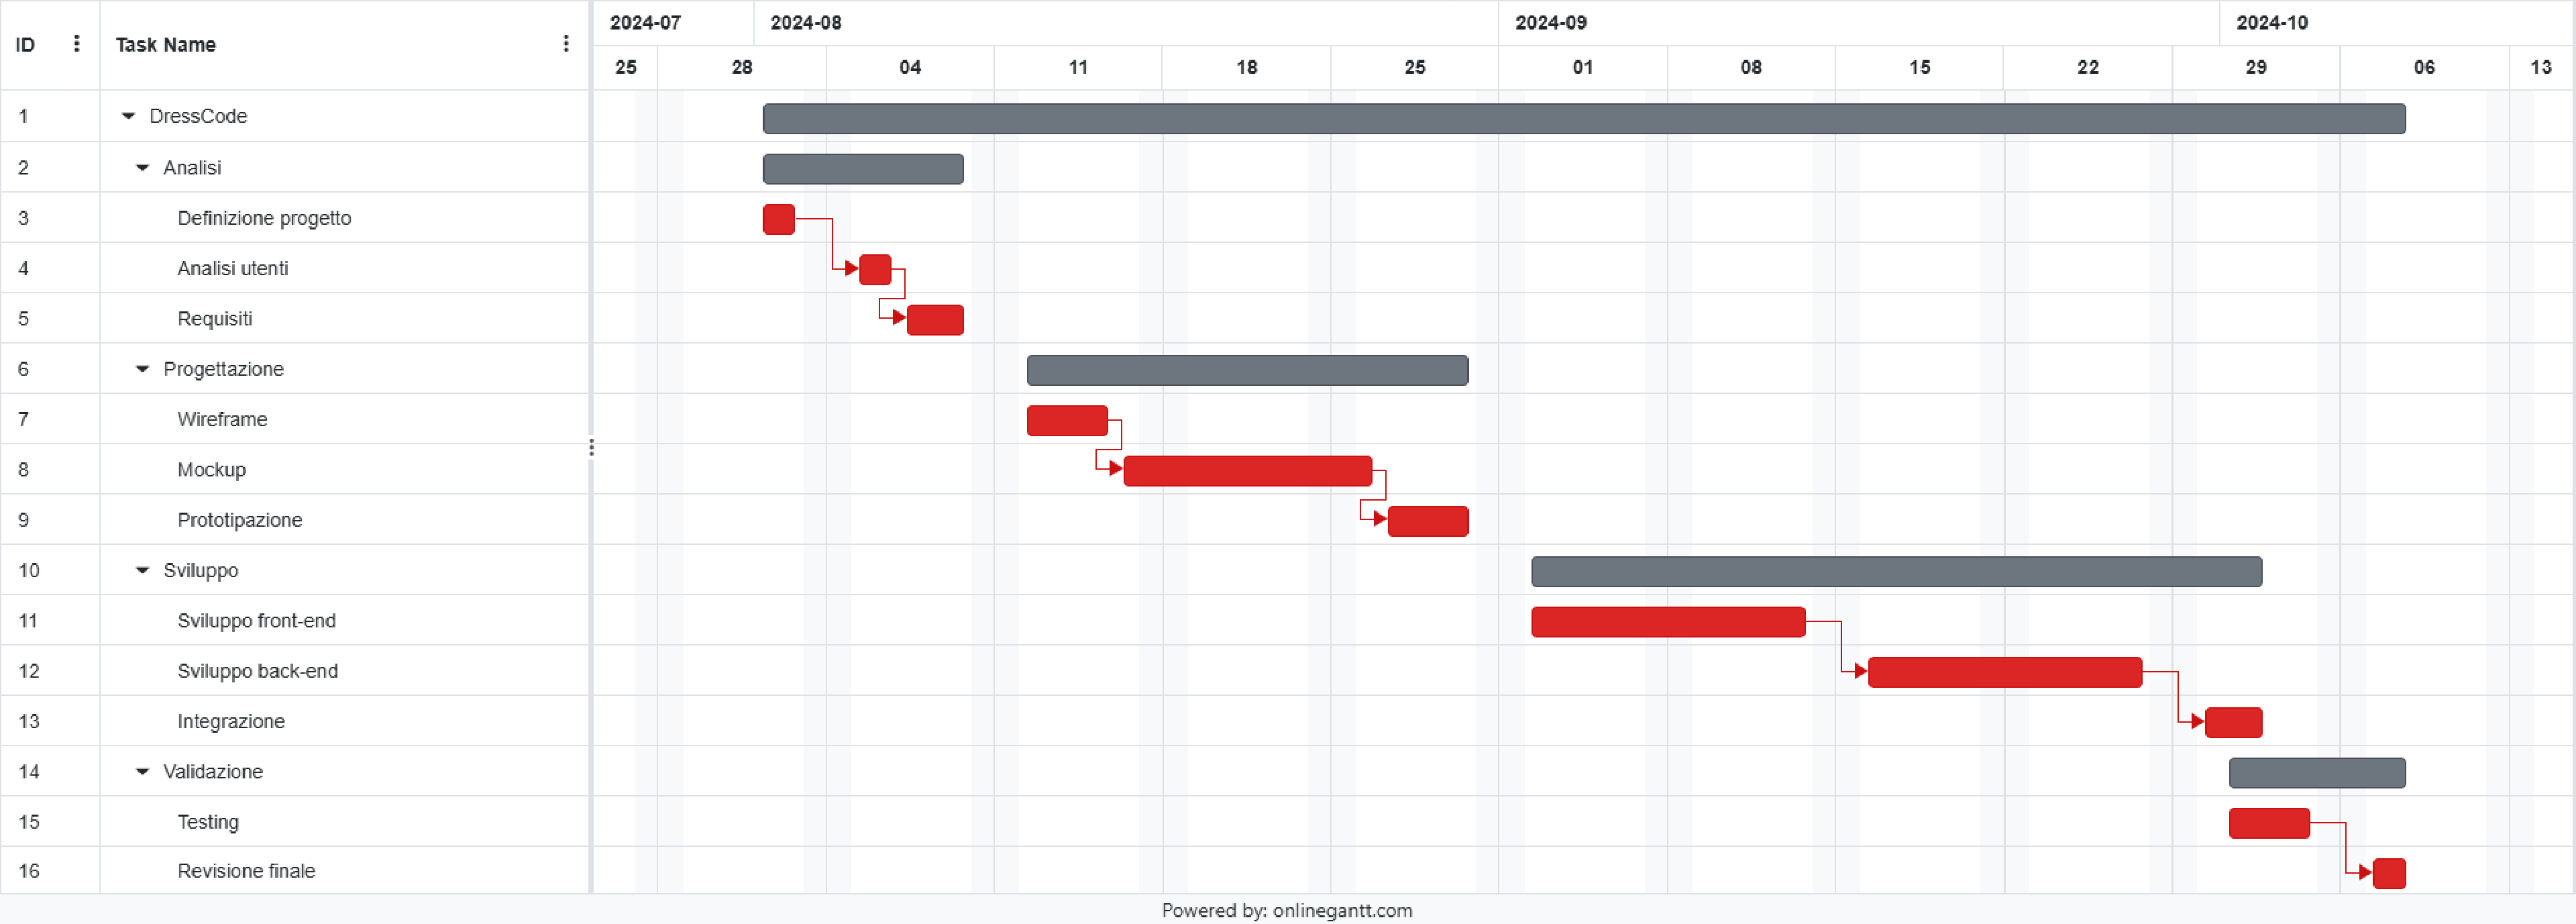
\includegraphics[width=1.4\linewidth,angle=-90]{gantt.pdf}
\end{center}

\subsection{Stima dei Costi e del Budget}
La stima dei costi per \textbf{DressCode} si basa sui 48 giorni lavorativi pianificati (1° agosto 2024 - 8 ottobre 2024), con Giorgio Matacera come unica risorsa. Assumendo 8 ore al giorno e un costo orario di 30 €, le 384 ore totali generano un costo diretto di 11.520 €. Questo copre analisi (54 ore), progettazione (108 ore), sviluppo (184 ore) e validazione (38 ore).
\\\\
I costi indiretti includono hosting base (15 €) e un dominio (15 €), per un totale di 60 €. Strumenti come Angular e PostgreSQL sono gratuiti. Un buffer di contingenza del 15\% (1.728 €) è aggiunto per imprevisti.
\\\\
Il costo totale stimato è quindi di 13.278 €, adeguato per un prototipo accademico realizzato individualmente.

\subsection{Valutazione dei Rischi}
La valutazione dei rischi per \textbf{DressCode} considera potenziali ostacoli nello sviluppo di \textbf{DressCode} entro i 48 giorni lavorativi pianificati (1° agosto 2024 - 8 ottobre 2024), con Giorgio Matacera come unica risorsa. Di seguito i principali rischi identificati e le strategie di mitigazione.
\\\\
Un rischio significativo è il ritardo nella consegna, dato il tempo limitato e il carico di lavoro su una sola persona. Per mitigare, si adotterà una metodologia agile con iterazioni brevi e priorità alle funzionalità essenziali. Un altro rischio è la complessità tecnica, specialmente nell'implementazione dell'editor drag-and-drop con Angular e dell'integrazione con PostgreSQL. Si affronterà usando librerie consolidate e test incrementali.
\\\\
Errori nel prototipo, come bug nell'esportazione dei form o nella collaborazione in tempo reale, potrebbero emergere. Si preverranno con sessioni di testing regolari durante lo sviluppo. Inoltre, la mancanza di risorse esterne (es. collaboratori o budget per strumenti premium) potrebbe limitare la scalabilità. Questo sarà gestito concentrandosi su un prototipo minimo viable (MVP) adatto al contesto accademico.
\\\\
Infine, un'interruzione personale (es. malattia) potrebbe influire sulla tabella di marcia. Si mitigherà pianificando un margine di contingenza del 15\% nel tempo e nel costo, già incluso nella stima di 13.308 €.

\usetikzlibrary{positioning}
\newcolumntype{M}{>{\centering\let\newline\\\arraybackslash\hspace{0pt}}m{1.5cm}}

\section{\huge Analisi degli Stakeholder}

\subsection{Introduzione}

Questo documento identifica e analizza gli stakeholder del progetto \textbf{DressCode}, che mira a sviluppare \textbf{DressCode}, un applicativo web per la creazione di moduli personalizzati. L'analisi degli stakeholder è fondamentale per integrare le esigenze di tutte le parti interessate nel processo di sviluppo, garantendo un prodotto che soddisfi sia gli obiettivi tecnici che quelli di user experience.

\subsection{Identificazione degli Stakeholder}
\subsubsection{Stakeholder Interni}
\begin{tabularx}{\textwidth}{|>{\centering\arraybackslash}l|>{\centering\arraybackslash}X|>{\centering\arraybackslash}X|>{\centering\arraybackslash}l|}
\hline
\rowcolor{Primary}
\textcolor{white}{\textbf{Stakeholder}} & 
\textcolor{white}{\textbf{Ruolo}} & 
\textcolor{white}{\textbf{Interessi}} & 
\textcolor{white}{\makecell{\textbf{Livello di} \\ \textbf{Influenza}}} \\ \hline
\textbf{Designer UX} & Responsabile della progettazione UX e gestione del progetto & Creare un'esperienza utente intuitiva e tematica & Alto \\ \hline
\textbf{Team di Sviluppo} & Sviluppatori frontend e backend & Realizzare un applicativo funzionale e scalabile & Alto \\ \hline
\end{tabularx}

\subsubsection{Stakeholder Esterni}
\begin{tabularx}{\textwidth}{|>{\centering\arraybackslash}l|>{\centering\arraybackslash}X|>{\centering\arraybackslash}X|>{\centering\arraybackslash}l|}
\hline
\rowcolor{Primary}
\textcolor{white}{\textbf{Stakeholder}} & 
\textcolor{white}{\textbf{Ruolo}} & 
\textcolor{white}{\textbf{Interessi}} & 
\textcolor{white}{\makecell{\textbf{Livello di} \\ \textbf{Influenza}}} \\ \hline
\textbf{Utenti Finali} & Sviluppatori web, designer, PMI & Facilità d'uso, personalizzazione dei form & Alto \\ \hline
\textbf{Partner Tecnologici} & Fornitori di hosting o API & Integrazione fluida con i loro servizi & Medio \\ \hline
\textbf{Concorrenza} & Altri form builder (es. Google Forms) & Monitorare innovazioni e posizionamento & Medio \\ \hline
\end{tabularx}

\subsection{Analisi}

\subsubsection{Designer UX}
\begin{itemize}
\item Interessi: Progettare un'interfaccia intuitiva e creativa basata sul tema dell'abbigliamento, rispettando i requisiti del corso di UX Design \& Process Architect. Garantire che il progetto soddisfi gli obiettivi di usabilità e innovazione. \\
\item Strategia di Coinvolgimento: Gestione diretta del progetto, con pianificazione e documentazione dettagliata per monitorare i progressi.
\end{itemize}

\subsubsection{Team di Sviluppo}
\begin{itemize}
\item Interessi: Implementare le funzionalità di \textbf{DressCode} (es. creazione di Vestiti, Tessuti, Trame, Fili, Fibre) in modo efficiente, con un codice pulito e scalabile. \\
\item Strategia di Coinvolgimento: Riunioni regolari per definire specifiche tecniche e ricevere feedback sul prototipo.
\end{itemize}

\subsubsection{Utenti Finali}
\begin{itemize}
\item Interessi: Creare moduli personalizzati rapidamente, con un'interfaccia user-friendly e opzioni di design (es. Accessori). Desiderano integrare i form in siti o applicazioni esterne senza difficoltà. \\
\item Strategia di Coinvolgimento: Raccolta di feedback tramite test utente sul prototipo per migliorare l'esperienza.
\end{itemize}

\subsubsection{Partner Tecnologici}
\begin{itemize}
\item Interessi: Garantire che \textbf{DressCode} si integri con i loro servizi (es. hosting per la Vetrina, API per la condivisione). \\
\item Strategia di Coinvolgimento: Collaborazione per test di compatibilità e documentazione tecnica condivisa.
\end{itemize}

\subsubsection{Concorrenza}
\begin{itemize}
\item Interessi: Osservare come \textbf{DressCode} si posiziona nel mercato rispetto a soluzioni esistenti, con un focus sul tema unico dell'abbigliamento. \\
\item Strategia di Coinvolgimento: Analisi comparativa per identificare punti di forza e differenziazione.
\end{itemize}

\pagebreak
\subsection{Strategia}
\begin{center}
\begin{tikzpicture}[xscale=1.5, yscale=1.5]
    \draw[thick,->] (-4,0) -- (4,0) node[fill=Secondary!40,right] {Interesse};
    \draw[thick,->] (0,-4) -- (0,4) node[fill=Secondary!40,above] {Influenza};

    \node[fill=Secondary!40,text width=2.612cm] at (4,4) {Alto Interesse\\Alta Influenza};
    \node[fill=Secondary!40,text width=2.851cm] at (-4,4) {Basso Interesse\\Alta Influenza};
    \node[fill=Secondary!40,text width=2.851cm] at (4,-4) {Alto Interesse\\Bassa Influenza};
    \node[fill=Secondary!40,text width=2.851cm] at (-4,-4) {Basso Interesse\\Bassa Influenza};

    \node[fill=Primary!40,draw=black,rounded corners] at (2,3.2) {Designer UX};
    \node[fill=Primary!40,draw=black,rounded corners] at (2,2.5) {Team di\\Sviluppo};
    \node[fill=Primary!40,draw=black,rounded corners] at (2,1.8) {Utenti Finali};
    \node[fill=Primary!20,draw=black,rounded corners] at (-2,2) {Partner\\Tecnologici};
    \node[fill=Primary!20,draw=black,rounded corners] at (1,-1) {Concorrenza};
\end{tikzpicture}
\end{center}

\subsubsection{Analisi della Concorrenza}
L'analisi della concorrenza per \textbf{DressCode} si concentra sui principali form builder web che competono con \textbf{DressCode}, un applicativo pensato per creare moduli personalizzati con un'interfaccia intuitiva e un tema ispirato all'abbigliamento. I concorrenti diretti includono strumenti consolidati come Google Forms e Typeform, mentre Jotform rappresenta un concorrente intermedio per funzionalità e personalizzazione.
\\\\
Google Forms offre un servizio gratuito e semplice, integrato con Google Workspace, ma manca di opzioni avanzate di design e di un'esperienza utente tematica, punti di forza di \textbf{DressCode}. Typeform si distingue per l'interfaccia moderna e interattiva, attirando utenti disposti a pagare per un'estetica curata, ma il suo costo (da 25 €/mese) e la complessità potrebbero scoraggiare piccole imprese o utenti base, un segmento che \textbf{DressCode} può intercettare con un'offerta più accessibile e distintiva. Jotform, con piani gratuiti e a pagamento (da 34 €/mese), compete su personalizzazione e integrazioni, ma non ha un'identità visiva unica come il tema abbigliamento di \textbf{DressCode}.
\\\\
Il vantaggio competitivo di \textbf{DressCode} risiede nella combinazione di semplicità, estetica tematica e integrazione facile, che lo differenzia da soluzioni generiche o eccessivamente complesse. Tuttavia, la concorrenza indiretta da piattaforme low-code come Wix o Squarespace, che includono moduli base nei loro editor, potrebbe attrarre utenti meno tecnici. Per superarli, \textbf{DressCode} punterà su un Minimum Viable Product (MVP) focalizzato su usabilità e branding unico, con potenziale espansione verso funzionalità collaborative.
\newcounter{requisiti}
\newcounter{vincoli}
\newcommand\numrequisiti{\stepcounter{requisiti}\arabic{requisiti}}
\newcommand\numvincoli{\stepcounter{vincoli}\arabic{vincoli}}
\newcommand\resetvincoli{\setcounter{vincoli}{0}}

\newcommand{\requisito}[3]{%
  \multicolumn{2}{|c|}{\cellcolor{Primary}\textcolor{white}{\textbf{REQ-DRESS-\numrequisiti\ -- #1}}} \\ \hline
  \textbf{Descrizione} & #2 \\ \hline
  \if\relax\detokenize{#3}\relax\else
  \textbf{Considerazioni} & #3 \\ \hline \fi
}
% Comando per i vincoli
\newcommand{\vincolo}[1]{%
  \textbf{VIN-DRESS-\arabic{requisiti}.\numvincoli} & #1 \\ \hline
}

\section{\huge Analisi dei Requisiti}
Questa sezione definisce i requisiti funzionali e non funzionali per \textbf{DressCode}', il form builder del progetto \textbf{DressCode}. I requisiti sono stati identificati considerando le esigenze degli utenti finali (sviluppatori web, designer, PMI) e gli obiettivi di semplicità, personalizzazione e integrazione del sistema.

\subsection{Requisiti Funzionali}
\begin{longtable}{|p{0.215\textwidth}|p{0.735\textwidth}|}
\hline
\requisito{Registrazione e Login Utente}{Il sistema deve consentire agli utenti di registrarsi e autenticarsi tramite email e password per accedere alla propria Boutique.}{Crittografia delle password con standard moderni (es. bcrypt).}
\vincolo{L'autenticazione deve essere implementata entro la prima iterazione del prototipo (2 settimane dall'inizio).}
\omit\resetvincoli

\requisito{Creazione di un Vestito}{Gli utenti devono poter creare un nuovo progetto (Vestito) che contenga gruppi di moduli (Tessuti).}{Supporto per denominazione personalizzata e categorizzazione dei Vestiti.}
\omit\resetvincoli

\requisito{Gestione dei Tessuti}{L'utente deve poter organizzare i moduli in gruppi logici (Tessuti) all'interno di un Vestito.}{Possibilità di riordinare o eliminare Tessuti.}
\omit\resetvincoli

\requisito{Definizione di Trame}{Gli utenti devono poter creare flussi di moduli (Trame) con sequenze logiche di Fili.}{Supporto per flussi condizionali (es. “se sì, vai al modulo X”).}
\omit\resetvincoli

\requisito{Creazione di Fili}{Il sistema deve permettere la creazione di singoli moduli (Fili) tramite un editor drag-and-drop.}{Offrire template predefiniti per moduli comuni (es. contatto, registrazione).}
\vincolo{L'editor drag-and-drop deve essere realizzato con Angular per compatibilità con il framework scelto.}
\omit\resetvincoli

\requisito{Personalizzazione Fibre}{Gli utenti devono poter aggiungere e configurare campi (Fibre) come testo, checkbox, dropdown, ecc.}{Anteprima in tempo reale delle modifiche.}
\omit\resetvincoli

\requisito{Esportazione Form}{I moduli creati devono essere esportabili come codice embeddable (es. HTML/JavaScript) per l'integrazione in siti esterni.}{Supporto per copia rapida del codice generato.}
\omit\resetvincoli

\requisito{Pubblicazione in Vetrina}{Gli utenti devono poter rendere pubblici i propri form nella Vetrina del sistema.}{Opzione per impostare visibilità pubblica o privata.}
\vincolo{La Vetrina deve essere disponibile solo agli utenti registrati nella versione prototipo.}
\omit\resetvincoli

\requisito{Integrazione API}{Possibilità di collegare i form a API esterne per inviare o ricevere dati.}{Documentazione chiara e esempi di integrazione.}
\omit\resetvincoli

\requisito{Analisi Statistiche}{Gli utenti devono poter visualizzare statistiche sull'uso dei loro form (es. numero di compilazioni) tramite una dashboard.}{Integrazione opzionale con strumenti come Google Analytics.}
\omit\resetvincoli

\requisito{Collaborazione}{Supporto per più utenti che lavorano sullo stesso Vestito in tempo reale.}{Notifiche delle modifiche e gestione dei conflitti.}
\vincolo{La collaborazione deve avere granularità fino ai flussi di moduli (Trame), solo 1 utente per volta potrà modificare un form (Filo).}
\omit\resetvincoli

\requisito{Notifiche Utente}{Inviare email per eventi chiave (es. pubblicazione in Vetrina, scadenza hosting).}{Personalizzazione delle preferenze di notifica.}
\omit\resetvincoli

\requisito{Gestione Media}{Gli utenti devono poter caricare immagini o altri media nei form.}{Compressione automatica per ottimizzare le prestazioni.}
\omit\resetvincoli

\requisito{Personalizzazione Accessori}{Gli utenti devono poter applicare temi estetici (Accessori) come colori e font ai form.}{Salvataggio dei temi personalizzati per riutilizzo.}
\omit\resetvincoli

\requisito{Cucitura Automatica}{Il sistema deve consentire agli utenti di unire moduli preesistenti (Cucitura) per creare Trame complesse.}{Suggerimenti automatici per combinazioni logiche.}
\omit\resetvincoli

\requisito{Sfilata}{Gli utenti devono poter mostrare i propri form in una modalità “Sfilata” con votazioni pubbliche.}{Integrazione con la Vetrina per promuovere i migliori form.}
\omit\resetvincoli

\requisito{Pianificazione Form}{Gli utenti devono poter programmare l'attivazione o disattivazione dei form in date specifiche.}{Interfaccia calendario per la gestione temporale.}
\omit\resetvincoli
\hline
\end{longtable}

\subsection{Requisiti Non Funzionali}
\begin{longtable}{|p{0.215\textwidth}|p{0.735\textwidth}|}
\hline
\requisito{Responsive Design}{I form generati devono essere automaticamente ottimizzati per desktop e dispositivi mobili.}{Test automatici di compatibilità responsiva.}
\omit\resetvincoli

\requisito{Accessibilità}{I form creati devono rispettare gli standard WCAG 2.1 per l'accessibilità.}{Fornire suggerimenti automatici per migliorare la conformità.}
\omit\resetvincoli

\requisito{Backup Automatici}{Il sistema deve salvare periodicamente i Vestiti e i relativi dati.}{Opzione per ripristinare versioni precedenti.}
\vincolo{Il database deve utilizzare PostgreSQL come specificato nell'analisi tecnica.}
\omit\resetvincoli

\requisito{SEO per Form Pubblici}{I form nella Vetrina devono essere ottimizzati per i motori di ricerca.}{Metadati configurabili (es. titolo, descrizione).}
\omit\resetvincoli

\requisito{Assistenza Tecnica}{Fornire supporto tramite chat o ticket per problemi tecnici.}{Tempi di risposta entro 24 ore.}
\vincolo{Il supporto tecnico deve essere simulato nel prototipo, senza implementazione reale.}
\omit\resetvincoli

\requisito{Scalabilità}{Il sistema deve supportare fino a 100 utenti simultanei nella fase prototipo.}{Scalabilità completa non richiesta per il corso.}
\omit\resetvincoli

\requisito{Usabilità}{L'interfaccia deve essere intuitiva per utenti senza competenze tecniche avanzate.}{Il tema dell'abbigliamento deve facilitare la comprensione dei concetti (es. Vestito, Trama).}
\omit\resetvincoli

\requisito{Sicurezza}{I dati degli utenti e dei form devono essere protetti tramite crittografia e autenticazione sicura.}{Rispetto del GDPR per la gestione dei dati personali.}
\vincolo{La crittografia deve essere implementata con standard AES-256 per i dati sensibili.}
\omit\resetvincoli

\requisito{Performance}{I form generati devono caricarsi in meno di 2 secondi su connessioni standard.}{Ottimizzazione delle risorse (es. compressione media).}
\omit\resetvincoli

\requisito{Compatibilità Browser}{I form devono funzionare correttamente sui principali browser (Chrome, Firefox, Safari, Edge).}{Test multipiattaforma automatizzati.}
\omit\resetvincoli

\requisito{Manutenibilità}{Il codice del sistema deve essere modulare e ben documentato per futuri aggiornamenti.}{Uso di commenti e struttura MVC in Angular.}
\omit\resetvincoli
\hline
\end{longtable}


\section{\huge UML}
\subsection{Diagramma delle Classi}
\begin{center}
    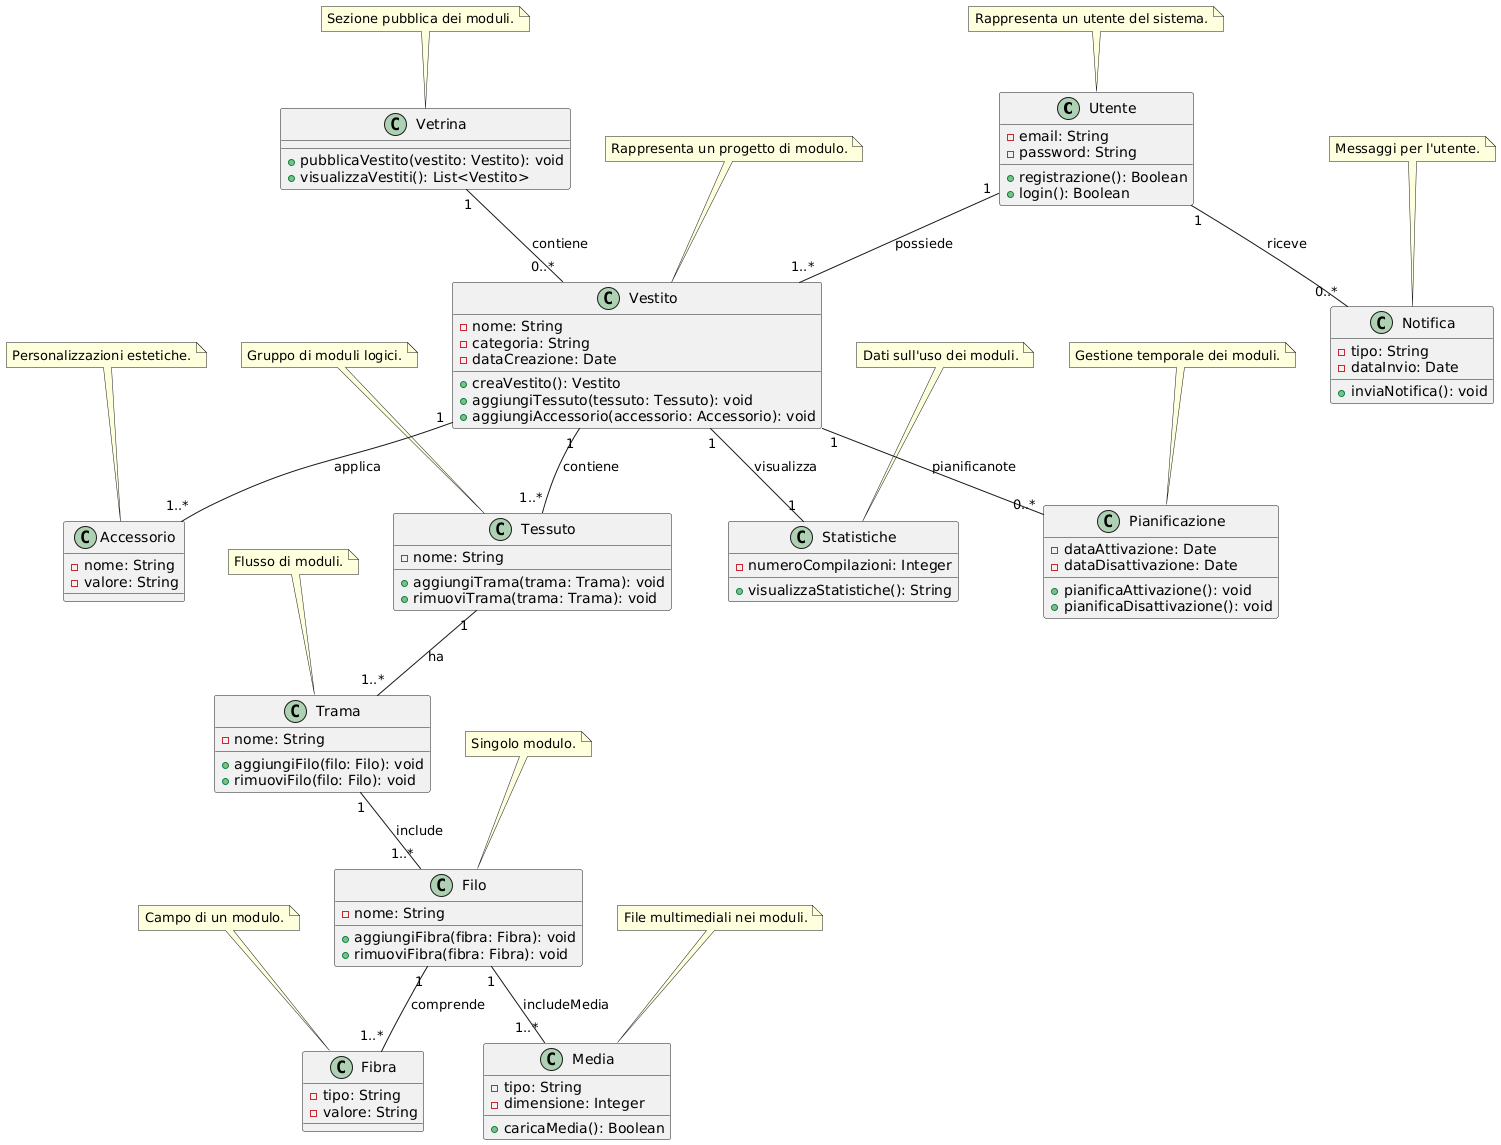
\includegraphics[width=1.3\linewidth,angle=-90]{uml/diagramma_delle_classi.png}
\end{center}
\subsection{Casi d'Uso}
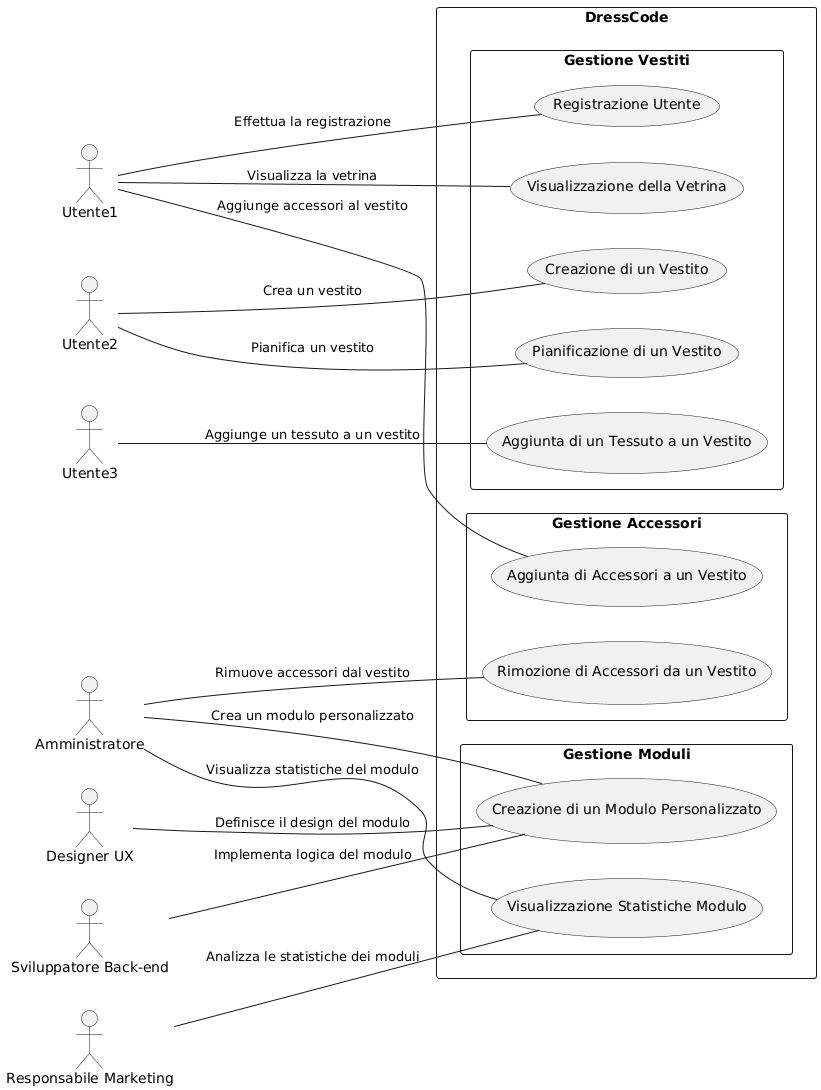
\includegraphics[width=1\linewidth]{uml/casi_d_uso.png}
\section{\huge Analisi degli Utenti}
L'analisi degli utenti per \textbf{DressCode} identifica i principali utilizzatori di \textbf{DressCode}, un costruttore di moduli web progettato per semplicità e personalizzazione con un tema abbigliamento. Tre gruppi emergono come target primari: sviluppatori web, designer grafici e piccole imprese (PMI).
\\\\
Gli sviluppatori web, spesso freelance o parte di team agili, cercano uno strumento rapido per creare moduli integrabili nei loro siti, valorizzando funzionalità come l'esportazione in HTML/JavaScript e l'editor avanzato. I designer grafici, abituati a strumenti visivi come Figma, apprezzano l'interfaccia intuitiva e la personalizzazione estetica (es. temi Accessori), ma potrebbero richiedere schemi predefiniti accattivanti. Le PMI, con competenze tecniche limitate, necessitano di un sistema facile da usare per moduli di contatto o sondaggi, privilegiando usabilità e pubblicazione diretta nella Vetrina.
\\\\
Questi utenti condividono l'esigenza di un'esperienza semplice e distintiva, che \textbf{DressCode} soddisfa con il suo approccio tematico e l'integrazione fluida. La sfida sarà bilanciare la semplicità per le PMI con le opzioni avanzate per sviluppatori e designer, testando il prototipo con ciascun gruppo.
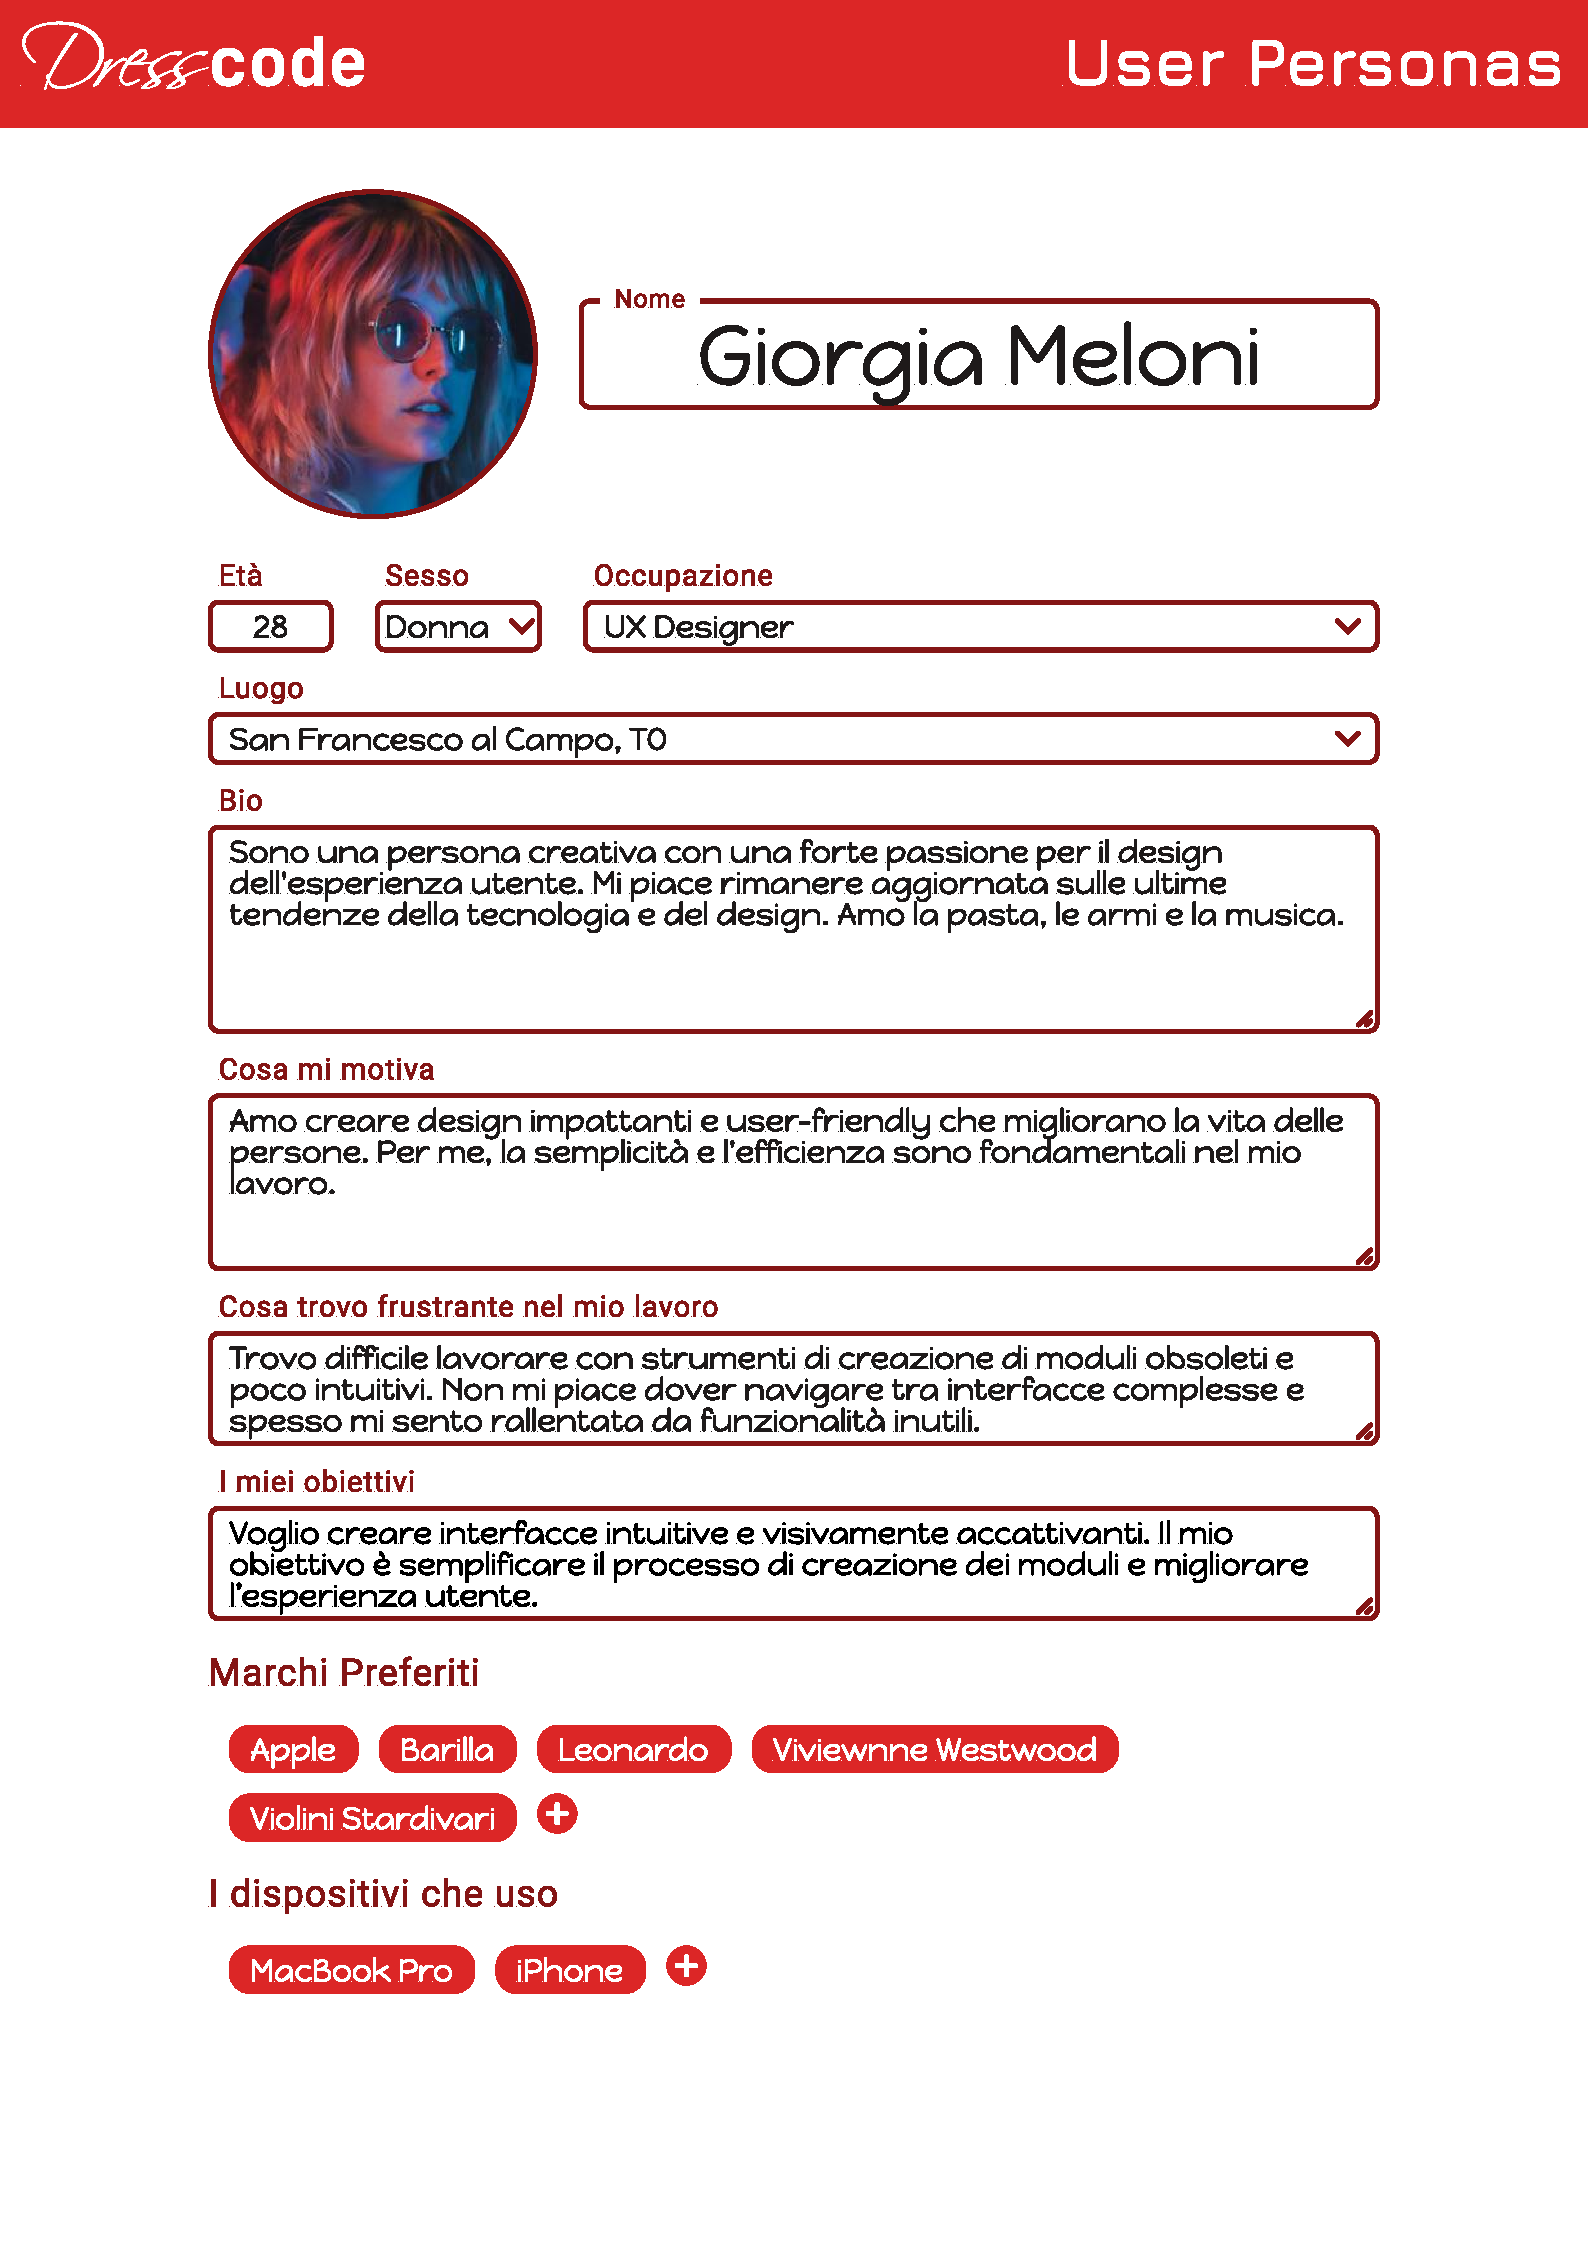
\includepdf[pages=-,pagecommand={}]{analisi degli utenti/personas_giorgia_meloni.pdf}
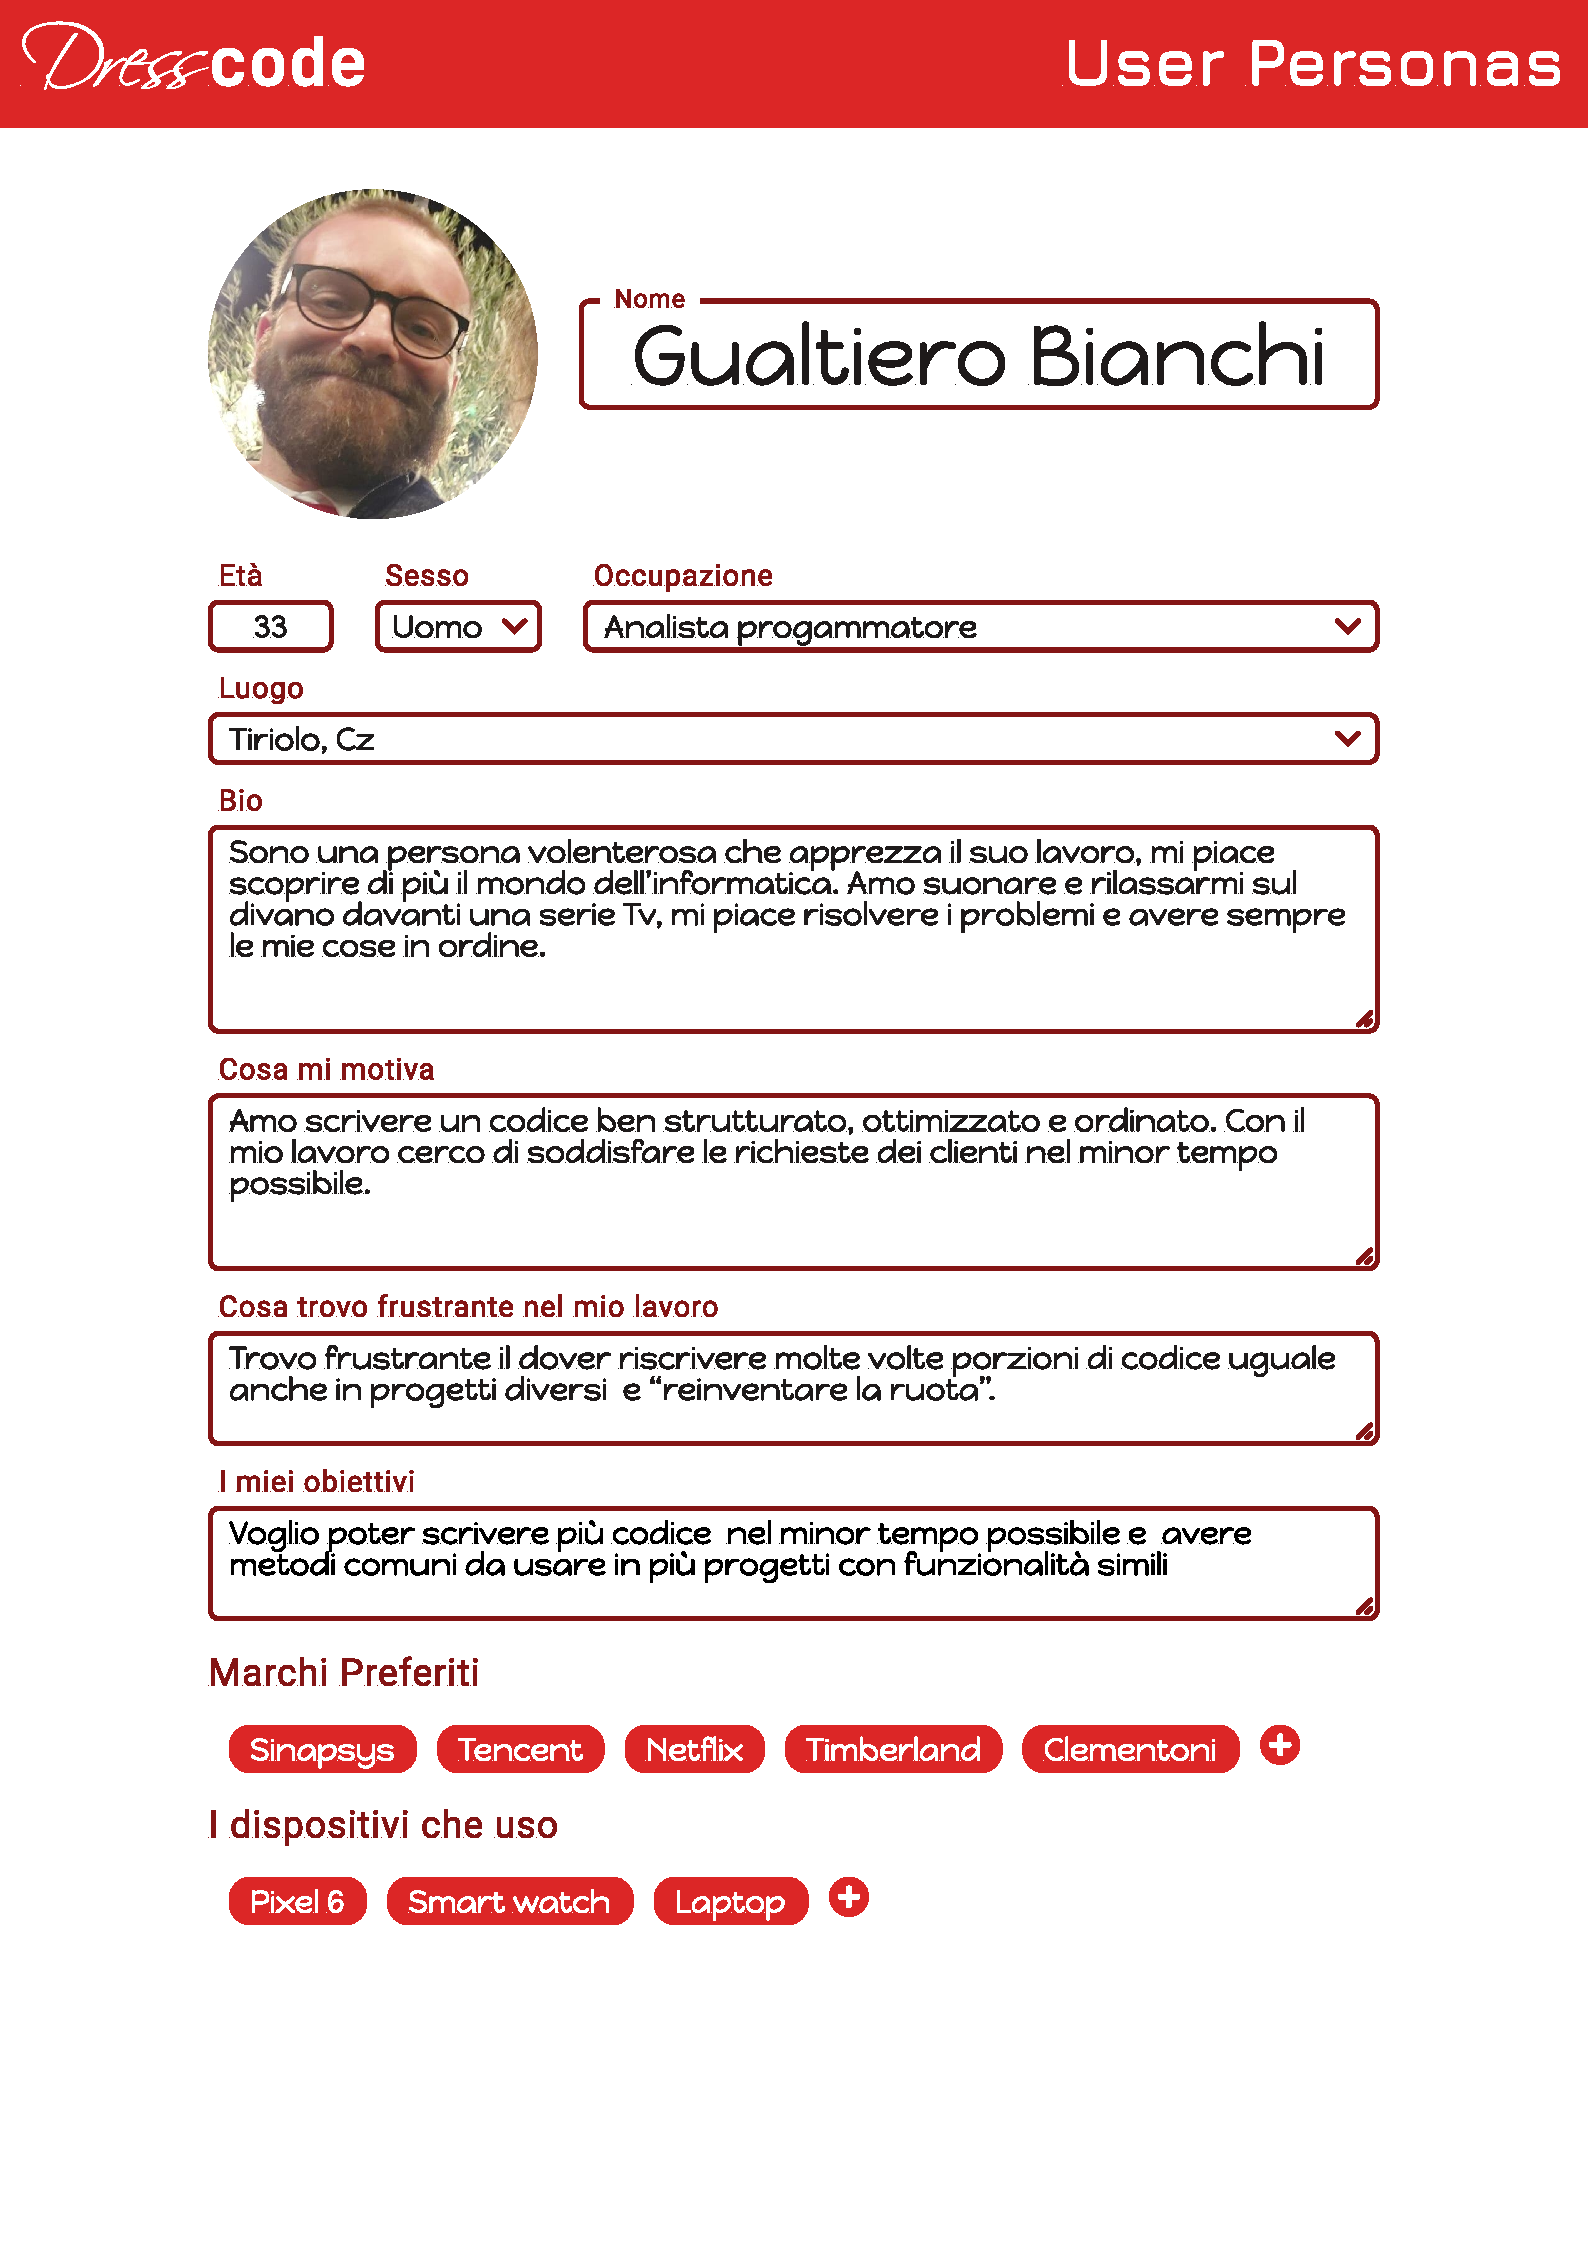
\includepdf[pages=-,pagecommand={}]{analisi degli utenti/personas_gualtiero_bianchi.pdf}

\section{Glossario}
\begin{tabularx}{\linewidth}{lX}
    \toprule
    \textbf{Termini} & \textbf{Definizione} \\
    \midrule
    Vestito & Progetto complessivo di un utente. \\
    Tessuto & Gruppo o cartella all'interno di un Vestito. \\
    Trama & Flusso di moduli con una sequenza logica. \\
    Filo & Singolo modulo all'interno di un flusso. \\
    Fibra & Campo specifico di un modulo. \\
    Boutique & Area personale dell'utente. \\
    Vetrina & Sezione pubblica per i form condivisi. \\
    \bottomrule
\end{tabularx}

\end{document}